\section{Results and Comparisons}
\label{sec:results}

\subsection{Equilibrium Intraband Benchmarks}
Our first validation step compares the numeric spectra generated by our energy-space integrator against the analytic closed-form correction derived in Section~\ref{sec:intraband}. As shown in Figure~\ref{fig:intra-eq}, the numeric results (blue solid line) perfectly overlay the analytic prediction (dashed red line) in the low-energy regime. Small deviations, manifest as a hardening of the spectrum at higher photon energies, are attributable to the full energy-dependent density of states $\rho(\mathcal{E}) \propto \sqrt{\mathcal{E}}$, which the constant-eDOS analytic approximation neglects. This agreement confirms the correctness of the thermal factor integration.

\begin{figure}[ht]
  \centering
  
\includegraphics[width=0.7\textwidth]{figures/stage_3_edos_vs_const_edos_heatmap.png}
  \caption{Comparison of equilibrium intraband emission calculation methods. The numeric integration with full eDOS (solid) is compared against the analytic constant-eDOS approximation (dashed). Deviations at high energies reflect the breakdown of the constant density of states assumption.}
  \label{fig:intra-eq}
\end{figure}

\subsection{Non-equilibrium Enhancement}
Under laser excitation, the electron distribution deviates from equilibrium, creating a "hot" smear of electrons above the Fermi energy and holes below it. Figure~\ref{fig:intra-noneq} illustrates the resulting emission spectra for varying degrees of non-equilibrium excitation, parameterized by the perturbation strength $\delta_E$. We observe a significant enhancement of the emission intensity, particularly around the Fermi edge where the product $f(1-f)$ is maximized. As the perturbation relaxes ($\delta_E \to 0$), the spectra smoothly recover the equilibrium baseline, demonstrating the stability of the non-equilibrium formalism.

\begin{figure}[ht]
  \centering
  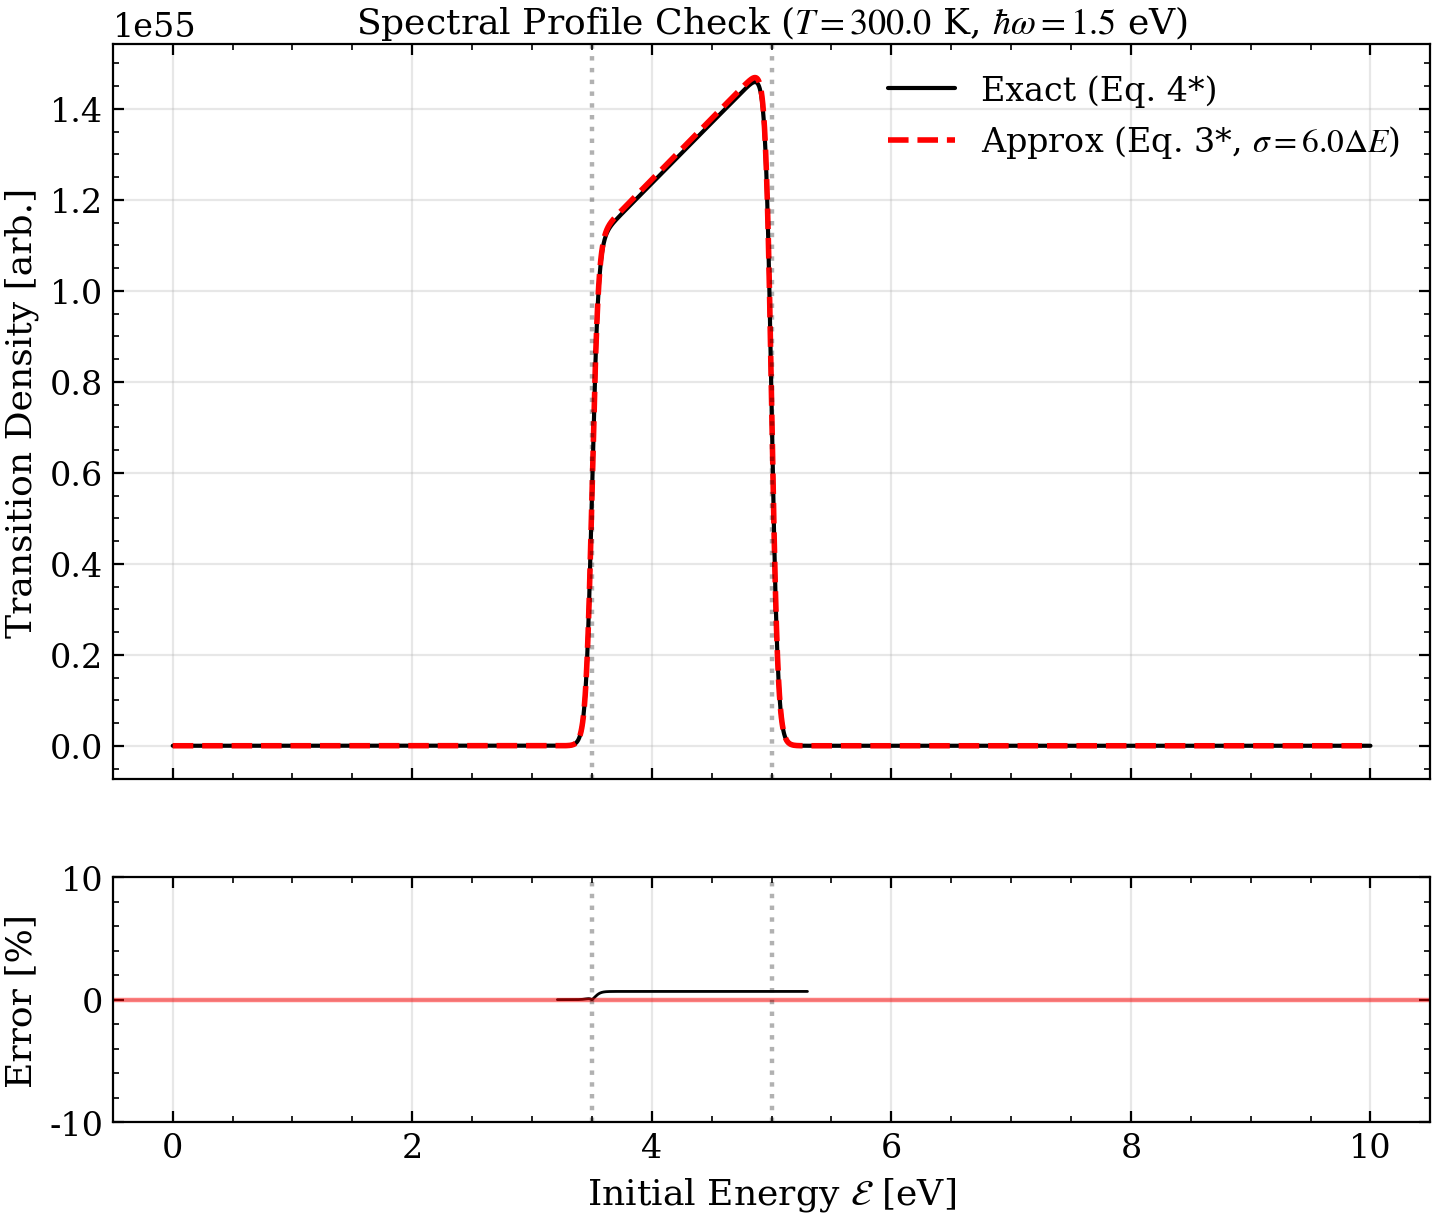
\includegraphics[width=0.7\textwidth]{figures/stage_4_spectral_profile.png}
  \caption{Non-equilibrium intraband emission spectra normalized to the peak intensity. The enhanced high-energy tail corresponds to the photo-excited hot carrier distribution.}
  \label{fig:intra-noneq}
\end{figure}

\subsection{Gaussian Delta Convergence}
Validating the multidimensional momentum-space integration requires ensuring that the Gaussian approximation of the energy delta function converges to the true delta limit. Figure~\ref{fig:delta} demonstrates this convergence behavior using a representative integrand. As the Gaussian width $\sigma$ decreases (moving left on the x-axis), the calculated integral value stabilizes, with the relative error dropping rapidly. This behavior validates the adaptive grid density strategy described in Section~\ref{sec:delta}, ensuring that our physical results are independent of the numeric regularization parameter.

\begin{figure}[ht]
  \centering
  
\includegraphics[width=0.6\textwidth]{figures/delta_convergence_cos.png}
  \caption{Convergence of the numerical integral as a function of the Gaussian delta width $\sigma$. The relative error decreases power-law fashion, stabilizing once the width is sufficiently small to resolve the integrand's features.}
  \label{fig:delta}
\end{figure}
